% Created by tikzDevice version 0.7.0 on 2014-04-28 15:35:23
% !TEX encoding = UTF-8 Unicode
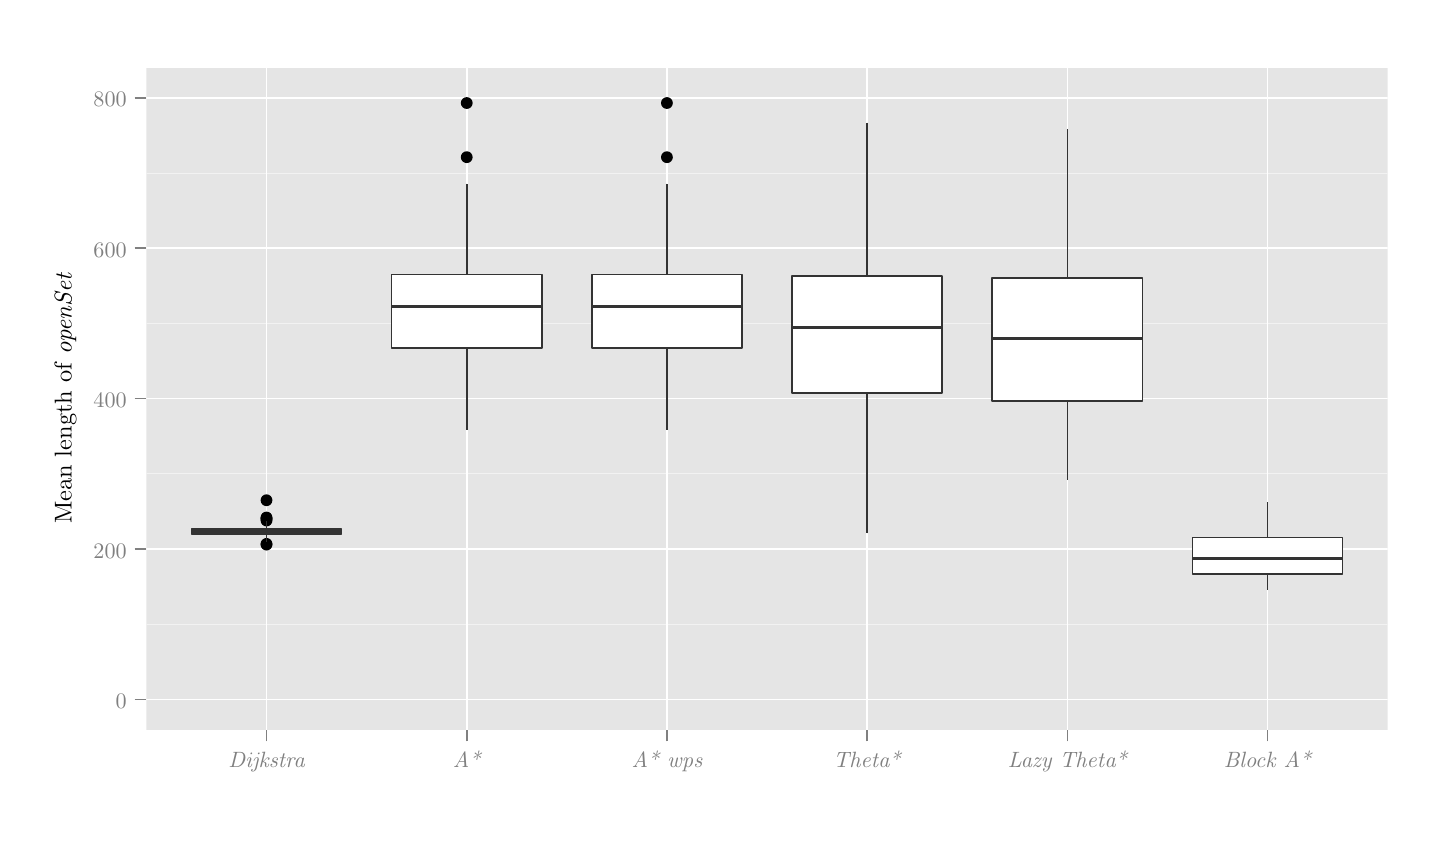
\begin{tikzpicture}[x=1pt,y=1pt]
\definecolor[named]{fillColor}{rgb}{1.00,1.00,1.00}
\path[use as bounding box,fill=fillColor,fill opacity=0.00] (0,0) rectangle (505.89,289.08);
\begin{scope}
\path[clip] (  0.00,  0.00) rectangle (505.89,289.08);
\definecolor[named]{drawColor}{rgb}{1.00,1.00,1.00}
\definecolor[named]{fillColor}{rgb}{1.00,1.00,1.00}

\path[draw=drawColor,line width= 0.6pt,line join=round,line cap=round,fill=fillColor] (  0.00, -0.00) rectangle (505.89,289.08);
\end{scope}
\begin{scope}
\path[clip] ( 42.90, 35.41) rectangle (491.44,274.63);
\definecolor[named]{fillColor}{rgb}{0.90,0.90,0.90}

\path[fill=fillColor] ( 42.90, 35.41) rectangle (491.44,274.63);
\definecolor[named]{drawColor}{rgb}{0.95,0.95,0.95}

\path[draw=drawColor,line width= 0.3pt,line join=round] ( 42.90, 73.47) --
	(491.44, 73.47);

\path[draw=drawColor,line width= 0.3pt,line join=round] ( 42.90,127.83) --
	(491.44,127.83);

\path[draw=drawColor,line width= 0.3pt,line join=round] ( 42.90,182.20) --
	(491.44,182.20);

\path[draw=drawColor,line width= 0.3pt,line join=round] ( 42.90,236.57) --
	(491.44,236.57);
\definecolor[named]{drawColor}{rgb}{1.00,1.00,1.00}

\path[draw=drawColor,line width= 0.6pt,line join=round] ( 42.90, 46.28) --
	(491.44, 46.28);

\path[draw=drawColor,line width= 0.6pt,line join=round] ( 42.90,100.65) --
	(491.44,100.65);

\path[draw=drawColor,line width= 0.6pt,line join=round] ( 42.90,155.02) --
	(491.44,155.02);

\path[draw=drawColor,line width= 0.6pt,line join=round] ( 42.90,209.39) --
	(491.44,209.39);

\path[draw=drawColor,line width= 0.6pt,line join=round] ( 42.90,263.75) --
	(491.44,263.75);

\path[draw=drawColor,line width= 0.6pt,line join=round] ( 86.30, 35.41) --
	( 86.30,274.63);

\path[draw=drawColor,line width= 0.6pt,line join=round] (158.65, 35.41) --
	(158.65,274.63);

\path[draw=drawColor,line width= 0.6pt,line join=round] (230.99, 35.41) --
	(230.99,274.63);

\path[draw=drawColor,line width= 0.6pt,line join=round] (303.34, 35.41) --
	(303.34,274.63);

\path[draw=drawColor,line width= 0.6pt,line join=round] (375.68, 35.41) --
	(375.68,274.63);

\path[draw=drawColor,line width= 0.6pt,line join=round] (448.03, 35.41) --
	(448.03,274.63);
\definecolor[named]{fillColor}{rgb}{0.00,0.00,0.00}

\path[fill=fillColor] ( 86.30,102.28) circle (  2.13);

\path[fill=fillColor] ( 86.30,118.32) circle (  2.13);

\path[fill=fillColor] ( 86.30,111.52) circle (  2.13);

\path[fill=fillColor] ( 86.30,111.80) circle (  2.13);

\path[fill=fillColor] ( 86.30,112.07) circle (  2.13);

\path[fill=fillColor] ( 86.30,102.55) circle (  2.13);

\path[fill=fillColor] ( 86.30,110.98) circle (  2.13);
\definecolor[named]{drawColor}{rgb}{0.20,0.20,0.20}
\definecolor[named]{fillColor}{rgb}{0.20,0.20,0.20}

\path[draw=drawColor,line width= 0.6pt,line join=round,fill=fillColor] ( 86.30,107.99) -- ( 86.30,110.71);

\path[draw=drawColor,line width= 0.6pt,line join=round,fill=fillColor] ( 86.30,106.09) -- ( 86.30,103.37);
\definecolor[named]{fillColor}{rgb}{1.00,1.00,1.00}

\path[draw=drawColor,line width= 0.6pt,line join=round,line cap=round,fill=fillColor] ( 59.17,107.99) --
	( 59.17,106.09) --
	(113.43,106.09) --
	(113.43,107.99) --
	( 59.17,107.99) --
	cycle;
\definecolor[named]{fillColor}{rgb}{0.20,0.20,0.20}

\path[draw=drawColor,line width= 1.1pt,line join=round,fill=fillColor] ( 59.17,106.90) -- (113.43,106.90);
\definecolor[named]{fillColor}{rgb}{0.00,0.00,0.00}

\path[fill=fillColor] (158.65,261.85) circle (  2.13);

\path[fill=fillColor] (158.65,242.28) circle (  2.13);
\definecolor[named]{fillColor}{rgb}{0.20,0.20,0.20}

\path[draw=drawColor,line width= 0.6pt,line join=round,fill=fillColor] (158.65,199.87) -- (158.65,232.76);

\path[draw=drawColor,line width= 0.6pt,line join=round,fill=fillColor] (158.65,173.37) -- (158.65,143.87);
\definecolor[named]{fillColor}{rgb}{1.00,1.00,1.00}

\path[draw=drawColor,line width= 0.6pt,line join=round,line cap=round,fill=fillColor] (131.52,199.87) --
	(131.52,173.37) --
	(185.78,173.37) --
	(185.78,199.87) --
	(131.52,199.87) --
	cycle;
\definecolor[named]{fillColor}{rgb}{0.20,0.20,0.20}

\path[draw=drawColor,line width= 1.1pt,line join=round,fill=fillColor] (131.52,188.18) -- (185.78,188.18);
\definecolor[named]{fillColor}{rgb}{0.00,0.00,0.00}

\path[fill=fillColor] (230.99,261.85) circle (  2.13);

\path[fill=fillColor] (230.99,242.28) circle (  2.13);
\definecolor[named]{fillColor}{rgb}{0.20,0.20,0.20}

\path[draw=drawColor,line width= 0.6pt,line join=round,fill=fillColor] (230.99,199.87) -- (230.99,232.76);

\path[draw=drawColor,line width= 0.6pt,line join=round,fill=fillColor] (230.99,173.37) -- (230.99,143.87);
\definecolor[named]{fillColor}{rgb}{1.00,1.00,1.00}

\path[draw=drawColor,line width= 0.6pt,line join=round,line cap=round,fill=fillColor] (203.86,199.87) --
	(203.86,173.37) --
	(258.12,173.37) --
	(258.12,199.87) --
	(203.86,199.87) --
	cycle;
\definecolor[named]{fillColor}{rgb}{0.20,0.20,0.20}

\path[draw=drawColor,line width= 1.1pt,line join=round,fill=fillColor] (203.86,188.18) -- (258.12,188.18);

\path[draw=drawColor,line width= 0.6pt,line join=round,fill=fillColor] (303.34,199.46) -- (303.34,254.78);

\path[draw=drawColor,line width= 0.6pt,line join=round,fill=fillColor] (303.34,157.06) -- (303.34,106.36);
\definecolor[named]{fillColor}{rgb}{1.00,1.00,1.00}

\path[draw=drawColor,line width= 0.6pt,line join=round,line cap=round,fill=fillColor] (276.21,199.46) --
	(276.21,157.06) --
	(330.47,157.06) --
	(330.47,199.46) --
	(276.21,199.46) --
	cycle;
\definecolor[named]{fillColor}{rgb}{0.20,0.20,0.20}

\path[draw=drawColor,line width= 1.1pt,line join=round,fill=fillColor] (276.21,180.57) -- (330.47,180.57);

\path[draw=drawColor,line width= 0.6pt,line join=round,fill=fillColor] (375.68,198.65) -- (375.68,252.34);

\path[draw=drawColor,line width= 0.6pt,line join=round,fill=fillColor] (375.68,154.20) -- (375.68,125.66);
\definecolor[named]{fillColor}{rgb}{1.00,1.00,1.00}

\path[draw=drawColor,line width= 0.6pt,line join=round,line cap=round,fill=fillColor] (348.55,198.65) --
	(348.55,154.20) --
	(402.81,154.20) --
	(402.81,198.65) --
	(348.55,198.65) --
	cycle;
\definecolor[named]{fillColor}{rgb}{0.20,0.20,0.20}

\path[draw=drawColor,line width= 1.1pt,line join=round,fill=fillColor] (348.55,176.77) -- (402.81,176.77);

\path[draw=drawColor,line width= 0.6pt,line join=round,fill=fillColor] (448.03,104.86) -- (448.03,117.50);

\path[draw=drawColor,line width= 0.6pt,line join=round,fill=fillColor] (448.03, 91.68) -- (448.03, 85.97);
\definecolor[named]{fillColor}{rgb}{1.00,1.00,1.00}

\path[draw=drawColor,line width= 0.6pt,line join=round,line cap=round,fill=fillColor] (420.90,104.86) --
	(420.90, 91.68) --
	(475.16, 91.68) --
	(475.16,104.86) --
	(420.90,104.86) --
	cycle;
\definecolor[named]{fillColor}{rgb}{0.20,0.20,0.20}

\path[draw=drawColor,line width= 1.1pt,line join=round,fill=fillColor] (420.90, 97.39) -- (475.16, 97.39);
\end{scope}
\begin{scope}
\path[clip] (  0.00,  0.00) rectangle (505.89,289.08);
\definecolor[named]{drawColor}{rgb}{0.50,0.50,0.50}

\node[text=drawColor,anchor=base east,inner sep=0pt, outer sep=0pt, scale=  0.80] at ( 35.78, 42.98) {0};

\node[text=drawColor,anchor=base east,inner sep=0pt, outer sep=0pt, scale=  0.80] at ( 35.78, 97.35) {200};

\node[text=drawColor,anchor=base east,inner sep=0pt, outer sep=0pt, scale=  0.80] at ( 35.78,151.71) {400};

\node[text=drawColor,anchor=base east,inner sep=0pt, outer sep=0pt, scale=  0.80] at ( 35.78,206.08) {600};

\node[text=drawColor,anchor=base east,inner sep=0pt, outer sep=0pt, scale=  0.80] at ( 35.78,260.45) {800};
\end{scope}
\begin{scope}
\path[clip] (  0.00,  0.00) rectangle (505.89,289.08);
\definecolor[named]{drawColor}{rgb}{0.50,0.50,0.50}

\path[draw=drawColor,line width= 0.6pt,line join=round] ( 38.63, 46.28) --
	( 42.90, 46.28);

\path[draw=drawColor,line width= 0.6pt,line join=round] ( 38.63,100.65) --
	( 42.90,100.65);

\path[draw=drawColor,line width= 0.6pt,line join=round] ( 38.63,155.02) --
	( 42.90,155.02);

\path[draw=drawColor,line width= 0.6pt,line join=round] ( 38.63,209.39) --
	( 42.90,209.39);

\path[draw=drawColor,line width= 0.6pt,line join=round] ( 38.63,263.75) --
	( 42.90,263.75);
\end{scope}
\begin{scope}
\path[clip] (  0.00,  0.00) rectangle (505.89,289.08);
\definecolor[named]{drawColor}{rgb}{0.50,0.50,0.50}

\path[draw=drawColor,line width= 0.6pt,line join=round] ( 86.30, 31.14) --
	( 86.30, 35.41);

\path[draw=drawColor,line width= 0.6pt,line join=round] (158.65, 31.14) --
	(158.65, 35.41);

\path[draw=drawColor,line width= 0.6pt,line join=round] (230.99, 31.14) --
	(230.99, 35.41);

\path[draw=drawColor,line width= 0.6pt,line join=round] (303.34, 31.14) --
	(303.34, 35.41);

\path[draw=drawColor,line width= 0.6pt,line join=round] (375.68, 31.14) --
	(375.68, 35.41);

\path[draw=drawColor,line width= 0.6pt,line join=round] (448.03, 31.14) --
	(448.03, 35.41);
\end{scope}
\begin{scope}
\path[clip] (  0.00,  0.00) rectangle (505.89,289.08);
\definecolor[named]{drawColor}{rgb}{0.50,0.50,0.50}

\node[text=drawColor,anchor=base,inner sep=0pt, outer sep=0pt, scale=  0.80] at ( 86.30, 21.69) {{\em Dijkstra}};

\node[text=drawColor,anchor=base,inner sep=0pt, outer sep=0pt, scale=  0.80] at (158.65, 21.69) {{\em A*}};

\node[text=drawColor,anchor=base,inner sep=0pt, outer sep=0pt, scale=  0.80] at (230.99, 21.69) {{\em A* wps}};

\node[text=drawColor,anchor=base,inner sep=0pt, outer sep=0pt, scale=  0.80] at (303.34, 21.69) {{\em Theta*}};

\node[text=drawColor,anchor=base,inner sep=0pt, outer sep=0pt, scale=  0.80] at (375.68, 21.69) {{\em Lazy Theta*}};

\node[text=drawColor,anchor=base,inner sep=0pt, outer sep=0pt, scale=  0.80] at (448.03, 21.69) {{\em Block A*}};
\end{scope}
\begin{scope}
\path[clip] (  0.00,  0.00) rectangle (505.89,289.08);
\definecolor[named]{drawColor}{rgb}{0.00,0.00,0.00}

\node[text=drawColor,rotate= 90.00,anchor=base,inner sep=0pt, outer sep=0pt, scale=  0.88] at ( 15.90,155.02) {Mean length of {\em openSet}};
\end{scope}
\end{tikzpicture}
